\chapter{Graph exploitation for software mining}%
\label{chp:graph-exploitation}

\TODO{Intro linking all the sections together.}

\section{Working with graph subsets}

So far, we have worked on compressed graph representations as a way to make
running analyses on the entire graph of development history manageable for
researchers using commodity hardware. While the compression ratio achieved is
impressive, the entire graph is often too computationally expensive to analyze
to be practical for many research use cases.  This is especially true for
prototyping, when the research is still at an exploratory stage and analysis
code is quickly iterated upon.

This problem can be addressed by providing less cumbersome \emph{graph
subsets}, i.e., smaller yet coherent collections of software artifacts which
can be used to perform analysis at a more reasonable scale. A tangentially
related problem of focusing analysis on a pre-narrowed logical subset of data,
i.e., only analyzing repositories matching some specific criteria, can also be
tackled by exporting ``subdatasets'' which only contain the relevant data to
process.

This section presents ways to provide subsets of the graph data in a way that
can be properly exploited for software mining, by leveraging the compressed
graph to select and export relevant software artifacts.

\subsection{Selecting artifacts of interest}

Evidently, to provide an exploitable subdataset of software development data,
it is not sufficient to uniformly extract random nodes from the graph. Doing so
would not preserve the logical structure linking software artifacts together
and make the graph extremely disconnected, which would render most of the
analysis results non-generalizable and of generally little value.
%
A better approach to generate logically coherent subdatasets is to always
export entire \emph{repositories} at once, i.e., the entire transitive closure
of a given set of origins. This minimizes the number of dangling links and
loose objects, and is generally an intuitive and expected way to construct
logical subsets of software mining data, as it closely matches the way the
entire dataset was built in the first place.

This reduces the artifact selection problem to selecting the list
\emph{origins} to be included in the subdataset.
Often, researchers will have a predetermined set of repositories of interest
(see \cref{sec:mining-selection-criteria}), which can be used to compute the
transitive closure of relevant artifacts. In other cases, the list of URLs
can be obtained externally using specific criteria, such as taking all the
repositories from a given hosting place, or all those with a minimum number of
stars. Finally, if the objective is to get a representative subset of origins
present in the archive, this can be achieved with uniform random sampling on
the list of origins in the archive.

To choose the appropriate number of origins to include in the subdataset, we
need a heuristic to estimate the size of the resulting graph given the number
of origins used to compute the transitive closure. Because of deduplication,
the size of the resulting graph does not scale linearly with the number of
origins: the more origins get included in the subgraph, the more likely it is
that the nodes in its transitive closure were already present from the closure
of another origin.

To attempt to measure this effect, we run an experiment on the entire
compressed graph: we (1) shuffle all the origins of the graph in a uniform
random order, (2) for each origin, lookup its transitive closure (3) once every
10k origins, tally the number of unique objects visited so far. The resulting
data is shown plotted in in \cref{fig:subdataset-size-function}.

\begin{figure}
    \centering
    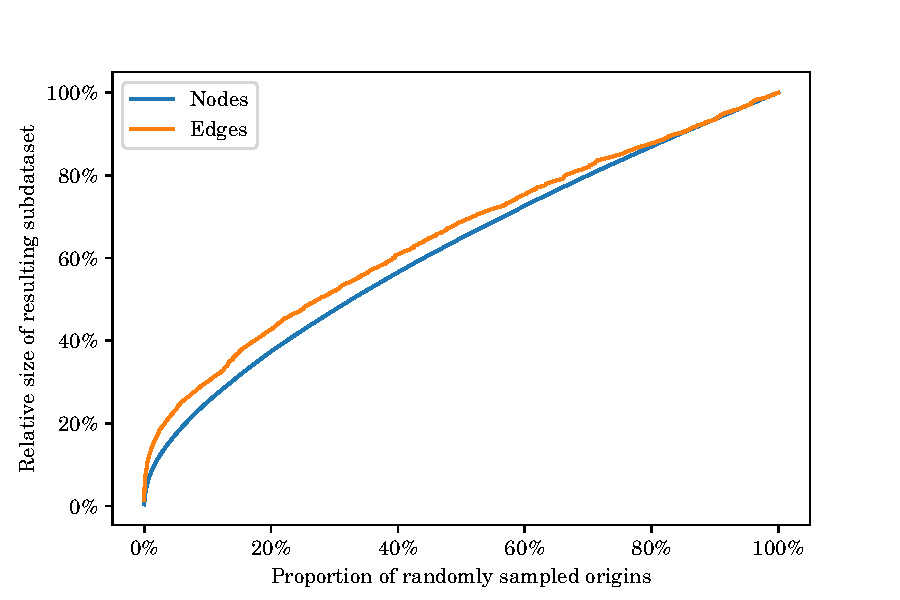
\includegraphics[width=0.8\textwidth]{img/graph-exploitation/subdataset_size_function}
    \caption{Proportion of nodes and edges obtained after sub-sampling the
        graph with a given number of origins. The x-axis represents the
        percentage of origins included in the subdataset; the y-axis represents
        the proportion of objects obtained in the resulting dataset.}%
    \label{fig:subdataset-size-function}
\end{figure}

As expected, the proportion of objects present in the resulting subdataset is
not proportional to the number of origins due to sharing effects. Instead,
the number of included objects has a sharp initial growth rate when few origins
have been visited, and this growth tapers off as a larger share of origins
has already been explored.

This data can be fitted in a logarithmic model of the form:

\[S(x) = a \log(1+bx^c)\]

A curve fitting algorithm minimizing the sum of squared residuals yields the
following coefficients for the subsampling heuristic, respectively for the
number of nodes and edges in the resulting subdataset:

\[
\begin{cases}
    S_V(x) = 500 \times \log(1 + 0.002 \times x ^{0.6}) \\
    S_E(x) = 250 \times \log(1 + 0.004 \times x ^{0.5}) \\
\end{cases}
\]

This model can be used to predict the size of the resulting dataset when
selecting a given sample size of origins, expressed as a proportion of the
total number of origins in the original dataset. As an example, if one wanted
to predict the number of nodes and edges in a subdataset containing a sample of
20\% of the total number of origins, replacing 20\% in the above model
predicts the following values:

\[
\begin{cases}
    S_V(20\%) = 500 \times \log(1 + 0.002 \times 0.2 ^{0.6}) = 38\% \\
    S_E(20\%) = 250 \times \log(1 + 0.004 \times 0.2 ^{0.5}) = 44\% \\
\end{cases}
\]

Therefore, a subdataset generated from a random sample of 20\% of the origins
will contain 38\% of the nodes and 44\% of the edges of the entire graph.
In order to target a specific amount of data in the subdataset (e.g., limiting
the size of the subdataset to less than \num{100000} nodes), the inverse of the
model can be used:

\[
\begin{cases}
    S_V^{-1}(x) = {\left(\cfrac{e^{\frac{x}{500}}-1}{0.002}\right)}^{\frac{1}{0.6}} \\
    S_E^{-1}(x) = {\left(\cfrac{e^{\frac{x}{250}}-1}{0.004}\right)}^{\frac{1}{0.5}} \\
\end{cases}
\]

Replacing $x$ in the model above with the target number of nodes or edges will
return a sample size of origins which is predicted to generate a subdataset
containing the given number of nodes or edges.

\subsection{Exporting subdatasets}

After having selected a subset of origins of interest (either with random
sampling or manual selection using various criteria), the next logical step is
to materialize the subdataset in a way that is suitable for a subsequent
analysis.
For this, we first need to compute the transitive closure of the set of all the
selected origins using the compressed graph. Once the subset of nodes has been
narrowed down, it becomes possible export the subdataset in the various formats
presented in \cref{chp:graph-dataset}.

By reading node and edge properties as described in
\cref{chp:graph-metadata}, it is relatively straightforward to export the
subdataset in the input edges format (\cref{sec:edges-format}), then recompress
it as a new graph using the graph compression pipeline
(\cref{chp:graph-compression}). The newly exported subgraph is then usable for
small-scale experiments.

Afterwards, the list of \glspl{SWHID} obtained from the compressed graph
traversal can be used to export the subdatasets in columnar format. Scale-out
processing tools like Amazon Athena can perform large JOINs to compute the
intersection between the full dataset and the set of \glspl{SWHID} of the
subdataset, and write the result in columnar format compatible with the
original graph dataset.

Using these techniques, we exported and made available a few ``teaser''
subdatasets containing a small set of origins selected using different
criteria, which can be used for prototyping with minimal hardware requirements.
These subdatasets illustrate different ways the \SWHGD{} can be used to build
exploitable datasets focused on narrowed data that is particularly relevant for
some specific research.

\paragraph{popular-4k} a subset of 4000 popular repositories from
GitHub, GitLab, PyPI and Debian. The selection criteria to pick the software
origins was the following:

\begin{itemize}
    \setlength\itemsep{0em}
    \item The 1000 most popular GitHub projects (by number of stars)
    \item The 1000 most popular Gitlab projects (by number of stars)
    \item The 1000 most popular PyPI projects (by usage statistics, according
        to the Top PyPI Packages
        database\footnote{\url{https://hugovk.github.io/top-pypi-packages/}}),
    \item The 1000 most popular Debian packages (by “votes” according to the
        Debian Popularity Contest
        database\footnote{\url{https://popcon.debian.org/}})
\end{itemize}

The resulting dataset is made available in the Apache Parquet and CSV formats,
with respective sizes of 23\,GiB and 27\,GiB, as well as on the Amazon Athena
query engine.

\paragraph{popular-python-3k} a subset of 3052 popular repositories tagged as
being written in the Python language from GitHub, GitLab, PyPI and Debian. The
selection criteria to pick the software origins was the following, similar to
popular-4k:

\begin{itemize}
    \setlength\itemsep{0em}
    \item The 1000 most popular GitHub projects written in Python (by number of
        stars)
    \item The 131 Gitlab projects written in Python which have 2 stars or more
    \item The 1000 most popular PyPI projects (by usage statistics, according
        to the Top PyPI Packages database)
    \item The 1000 most popular Debian packages with the debtag
        \texttt{implemented-in::python} (by “votes” according to the Debian
        Popularity Contest database)
\end{itemize}

The resulting dataset is made available in the Apache Parquet and CSV formats,
with respective sizes of 4.7\,GiB and 5.3\,GiB, as well as on the Amazon Athena
query engine.

\paragraph{gitlab-100k} a subset of \num{100000} repositories from GitLab,
hosted at the main \texttt{gitlab.com} instance, sampled using a uniform random
distribution. This dataset is made available as a compressed graph, containing
304 million nodes and 9.5 billion edges, for a total size of 6.8\,GiB (3.6\,GiB
for the direct graph and 3.2\,GiB for the transposed graph).

\paragraph{gitlab-all} a subset of every repository from GitLab, hosted at the
main \texttt{gitlab.com} instance. This dataset is made available as a
compressed graph, containing 1.0 billion nodes and 27.9 billion edges, for a
total size of 20.6\,GiB (9.6\,GiB for the direct graph and 11\,GiB for the
transposed graph).

\subsection{Overlay subgraphs}

While exporting entire subdatasets is extremely useful for a lot of research
use cases, as it reduces the size of the dataset so that it only contains the
relevant data for these needs, the process is quite slow. In particular, it is
not well suited to \TODO{}
